\documentclass[1p]{elsarticle_modified}
%\bibliographystyle{elsarticle-num}

%\usepackage[colorlinks]{hyperref}
%\usepackage{abbrmath_seonhwa} %\Abb, \Ascr, \Acal ,\Abf, \Afrak
\usepackage{amsfonts}
\usepackage{amssymb}
\usepackage{amsmath}
\usepackage{amsthm}
\usepackage{scalefnt}
\usepackage{amsbsy}
\usepackage{kotex}
\usepackage{caption}
\usepackage{subfig}
\usepackage{color}
\usepackage{graphicx}
\usepackage{xcolor} %% white, black, red, green, blue, cyan, magenta, yellow
\usepackage{float}
\usepackage{setspace}
\usepackage{hyperref}

\usepackage{tikz}
\usetikzlibrary{arrows}

\usepackage{multirow}
\usepackage{array} % fixed length table
\usepackage{hhline}

%%%%%%%%%%%%%%%%%%%%%
\makeatletter
\renewcommand*\env@matrix[1][\arraystretch]{%
	\edef\arraystretch{#1}%
	\hskip -\arraycolsep
	\let\@ifnextchar\new@ifnextchar
	\array{*\c@MaxMatrixCols c}}
\makeatother %https://tex.stackexchange.com/questions/14071/how-can-i-increase-the-line-spacing-in-a-matrix
%%%%%%%%%%%%%%%

\usepackage[normalem]{ulem}

\newcommand{\msout}[1]{\ifmmode\text{\sout{\ensuremath{#1}}}\else\sout{#1}\fi}
%SOURCE: \msout is \stkout macro in https://tex.stackexchange.com/questions/20609/strikeout-in-math-mode

\newcommand{\cancel}[1]{
	\ifmmode
	{\color{red}\msout{#1}}
	\else
	{\color{red}\sout{#1}}
	\fi
}

\newcommand{\add}[1]{
	{\color{blue}\uwave{#1}}
}

\newcommand{\replace}[2]{
	\ifmmode
	{\color{red}\msout{#1}}{\color{blue}\uwave{#2}}
	\else
	{\color{red}\sout{#1}}{\color{blue}\uwave{#2}}
	\fi
}

\newcommand{\Sol}{\mathcal{S}} %segment
\newcommand{\D}{D} %diagram
\newcommand{\A}{\mathcal{A}} %arc


%%%%%%%%%%%%%%%%%%%%%%%%%%%%%5 test

\def\sl{\operatorname{\textup{SL}}(2,\Cbb)}
\def\psl{\operatorname{\textup{PSL}}(2,\Cbb)}
\def\quan{\mkern 1mu \triangleright \mkern 1mu}

\theoremstyle{definition}
\newtheorem{thm}{Theorem}[section]
\newtheorem{prop}[thm]{Proposition}
\newtheorem{lem}[thm]{Lemma}
\newtheorem{ques}[thm]{Question}
\newtheorem{cor}[thm]{Corollary}
\newtheorem{defn}[thm]{Definition}
\newtheorem{exam}[thm]{Example}
\newtheorem{rmk}[thm]{Remark}
\newtheorem{alg}[thm]{Algorithm}

\newcommand{\I}{\sqrt{-1}}
\begin{document}

%\begin{frontmatter}
%
%\title{Boundary parabolic representations of knots up to 8 crossings}
%
%%% Group authors per affiliation:
%\author{Yunhi Cho} 
%\address{Department of Mathematics, University of Seoul, Seoul, Korea}
%\ead{yhcho@uos.ac.kr}
%
%
%\author{Seonhwa Kim} %\fnref{s_kim}}
%\address{Center for Geometry and Physics, Institute for Basic Science, Pohang, 37673, Korea}
%\ead{ryeona17@ibs.re.kr}
%
%\author{Hyuk Kim}
%\address{Department of Mathematical Sciences, Seoul National University, Seoul 08826, Korea}
%\ead{hyukkim@snu.ac.kr}
%
%\author{Seokbeom Yoon}
%\address{Department of Mathematical Sciences, Seoul National University, Seoul, 08826,  Korea}
%\ead{sbyoon15@snu.ac.kr}
%
%\begin{abstract}
%We find all boundary parabolic representation of knots up to 8 crossings.
%
%\end{abstract}
%\begin{keyword}
%    \MSC[2010] 57M25 
%\end{keyword}
%
%\end{frontmatter}

%\linenumbers
%\tableofcontents
%
\newcommand\colored[1]{\textcolor{white}{\rule[-0.35ex]{0.8em}{1.4ex}}\kern-0.8em\color{red} #1}%
%\newcommand\colored[1]{\textcolor{white}{ #1}\kern-2.17ex	\textcolor{white}{ #1}\kern-1.81ex	\textcolor{white}{ #1}\kern-2.15ex\color{red}#1	}

{\Large $\underline{11a_{101}~(K11a_{101})}$}

\setlength{\tabcolsep}{10pt}
\renewcommand{\arraystretch}{1.6}
\vspace{1cm}\begin{tabular}{m{100pt}>{\centering\arraybackslash}m{274pt}}
\multirow{5}{120pt}{
	\centering
	\includegraphics[width=112pt]{../../../GIT/diagram.site/Diagrams/png/350_11a_101.png}\\
\ \ \ A knot diagram\footnotemark}&
\allowdisplaybreaks
\textbf{Linearized knot diagam} \\
\cline{2-2}
 &
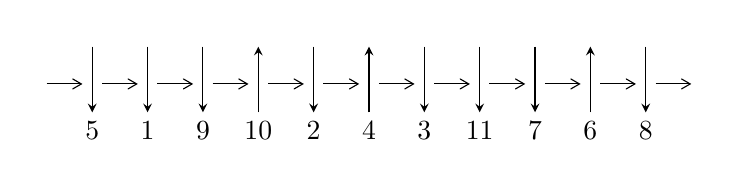
\begin{tikzpicture}[x=20pt, y=17pt]
	% nodes
	\node (C0) at (0, 0) {};
	\node (C1) at (1, 0) {};
	\node (C1U) at (1, +1) {};
	\node (C1D) at (1, -1) {5};

	\node (C2) at (2, 0) {};
	\node (C2U) at (2, +1) {};
	\node (C2D) at (2, -1) {1};

	\node (C3) at (3, 0) {};
	\node (C3U) at (3, +1) {};
	\node (C3D) at (3, -1) {9};

	\node (C4) at (4, 0) {};
	\node (C4U) at (4, +1) {};
	\node (C4D) at (4, -1) {10};

	\node (C5) at (5, 0) {};
	\node (C5U) at (5, +1) {};
	\node (C5D) at (5, -1) {2};

	\node (C6) at (6, 0) {};
	\node (C6U) at (6, +1) {};
	\node (C6D) at (6, -1) {4};

	\node (C7) at (7, 0) {};
	\node (C7U) at (7, +1) {};
	\node (C7D) at (7, -1) {3};

	\node (C8) at (8, 0) {};
	\node (C8U) at (8, +1) {};
	\node (C8D) at (8, -1) {11};

	\node (C9) at (9, 0) {};
	\node (C9U) at (9, +1) {};
	\node (C9D) at (9, -1) {7};

	\node (C10) at (10, 0) {};
	\node (C10U) at (10, +1) {};
	\node (C10D) at (10, -1) {6};

	\node (C11) at (11, 0) {};
	\node (C11U) at (11, +1) {};
	\node (C11D) at (11, -1) {8};
	\node (C12) at (12, 0) {};

	% arrows
	\draw[->,>={angle 60}]
	(C0) edge (C1) (C1) edge (C2) (C2) edge (C3) (C3) edge (C4) (C4) edge (C5) (C5) edge (C6) (C6) edge (C7) (C7) edge (C8) (C8) edge (C9) (C9) edge (C10) (C10) edge (C11) (C11) edge (C12) ;	\draw[->,>=stealth]
	(C1U) edge (C1D) (C2U) edge (C2D) (C3U) edge (C3D) (C4D) edge (C4U) (C5U) edge (C5D) (C6D) edge (C6U) (C7U) edge (C7D) (C8U) edge (C8D) (C9U) edge (C9D) (C10D) edge (C10U) (C11U) edge (C11D) ;
	\end{tikzpicture} \\
\hhline{~~} \\& 
\textbf{Solving Sequence} \\ \cline{2-2} 
 &
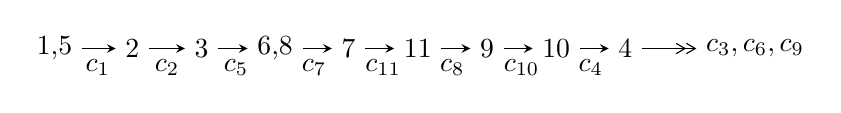
\begin{tikzpicture}[x=25pt, y=7pt]
	% node
	\node (A0) at (-1/8, 0) {1,5};
	\node (A1) at (1, 0) {2};
	\node (A2) at (2, 0) {3};
	\node (A3) at (49/16, 0) {6,8};
	\node (A4) at (33/8, 0) {7};
	\node (A5) at (41/8, 0) {11};
	\node (A6) at (49/8, 0) {9};
	\node (A7) at (57/8, 0) {10};
	\node (A8) at (65/8, 0) {4};
	\node (C1) at (1/2, -1) {$c_{1}$};
	\node (C2) at (3/2, -1) {$c_{2}$};
	\node (C3) at (5/2, -1) {$c_{5}$};
	\node (C4) at (29/8, -1) {$c_{7}$};
	\node (C5) at (37/8, -1) {$c_{11}$};
	\node (C6) at (45/8, -1) {$c_{8}$};
	\node (C7) at (53/8, -1) {$c_{10}$};
	\node (C8) at (61/8, -1) {$c_{4}$};
	\node (A9) at (10, 0) {$c_{3},c_{6},c_{9}$};

	% edge
	\draw[->,>=stealth]	
	(A0) edge (A1) (A1) edge (A2) (A2) edge (A3) (A3) edge (A4) (A4) edge (A5) (A5) edge (A6) (A6) edge (A7) (A7) edge (A8) ;
	\draw[->>,>={angle 60}]	
	(A8) edge (A9);
\end{tikzpicture} \\ 

\end{tabular} \\

\footnotetext{
The image of knot diagram is generated by the software ``\textbf{Draw programme}" developed by Andrew Bartholomew(\url{http://www.layer8.co.uk/maths/draw/index.htm\#Running-draw}), where we modified some parts for our purpose(\url{https://github.com/CATsTAILs/LinksPainter}).
}\phantom \\ \newline 
\centering \textbf{Ideals for irreducible components\footnotemark of $X_{\text{par}}$} 
 
\begin{align*}
I^u_{1}&=\langle 
-5.86190\times10^{189} u^{104}+3.24426\times10^{190} u^{103}+\cdots+1.28496\times10^{191} b+2.04597\times10^{191},\\
\phantom{I^u_{1}}&\phantom{= \langle  }-9.93421\times10^{190} u^{104}-1.87948\times10^{191} u^{103}+\cdots+5.39685\times10^{192} a-1.98703\times10^{193},\\
\phantom{I^u_{1}}&\phantom{= \langle  }u^{105}-3 u^{104}+\cdots+26 u-21\rangle \\
I^u_{2}&=\langle 
- u^{17}-4 u^{16}+\cdots+b-4,\;-10 u^{17}-12 u^{16}+\cdots+a-10,\;u^{18}+2 u^{17}+\cdots+2 u+1\rangle \\
I^u_{3}&=\langle 
- a^2+b- a,\;a^4+2 a^3+2 a^2+a+1,\;u-1\rangle \\
\\
\end{align*}
\raggedright * 3 irreducible components of $\dim_{\mathbb{C}}=0$, with total 127 representations.\\
\footnotetext{All coefficients of polynomials are rational numbers. But the coefficients are sometimes approximated in decimal forms when there is not enough margin.}
\newpage
\renewcommand{\arraystretch}{1}
\centering \section*{I. $I^u_{1}= \langle -5.86\times10^{189} u^{104}+3.24\times10^{190} u^{103}+\cdots+1.28\times10^{191} b+2.05\times10^{191},\;-9.93\times10^{190} u^{104}-1.88\times10^{191} u^{103}+\cdots+5.40\times10^{192} a-1.99\times10^{193},\;u^{105}-3 u^{104}+\cdots+26 u-21 \rangle$}
\flushleft \textbf{(i) Arc colorings}\\
\begin{tabular}{m{7pt} m{180pt} m{7pt} m{180pt} }
\flushright $a_{1}=$&$\begin{pmatrix}1\\0\end{pmatrix}$ \\
\flushright $a_{5}=$&$\begin{pmatrix}0\\u\end{pmatrix}$ \\
\flushright $a_{2}=$&$\begin{pmatrix}1\\u^2\end{pmatrix}$ \\
\flushright $a_{3}=$&$\begin{pmatrix}- u^2+1\\u^2\end{pmatrix}$ \\
\flushright $a_{6}=$&$\begin{pmatrix}- u\\- u^3+u\end{pmatrix}$ \\
\flushright $a_{8}=$&$\begin{pmatrix}0.0184074 u^{104}+0.0348256 u^{103}+\cdots-3.82299 u+3.68184\\0.0456192 u^{104}-0.252478 u^{103}+\cdots+11.7933 u-1.59224\end{pmatrix}$ \\
\flushright $a_{7}=$&$\begin{pmatrix}0.0754639 u^{104}-0.151948 u^{103}+\cdots+4.47496 u+3.26401\\0.0217419 u^{104}-0.195594 u^{103}+\cdots+13.2792 u-2.22961\end{pmatrix}$ \\
\flushright $a_{11}=$&$\begin{pmatrix}0.106302 u^{104}-0.0726312 u^{103}+\cdots-18.1193 u+6.55450\\-0.0367543 u^{104}-0.0382608 u^{103}+\cdots+0.133832 u+0.505694\end{pmatrix}$ \\
\flushright $a_{9}=$&$\begin{pmatrix}0.0375876 u^{104}+0.0739669 u^{103}+\cdots+2.09040 u+2.16319\\-0.123383 u^{104}+0.240256 u^{103}+\cdots-8.75520 u+3.25940\end{pmatrix}$ \\
\flushright $a_{10}=$&$\begin{pmatrix}0.00776219 u^{104}+0.0887609 u^{103}+\cdots-15.0253 u+5.17372\\-0.0721333 u^{104}+0.148940 u^{103}+\cdots-1.53959 u-0.932304\end{pmatrix}$ \\
\flushright $a_{4}=$&$\begin{pmatrix}-0.0513625 u^{104}+0.118285 u^{103}+\cdots+16.1435 u-2.45451\\0.00759574 u^{104}+0.0691986 u^{103}+\cdots-13.0165 u+3.52395\end{pmatrix}$\\ \flushright $a_{4}=$&$\begin{pmatrix}-0.0513625 u^{104}+0.118285 u^{103}+\cdots+16.1435 u-2.45451\\0.00759574 u^{104}+0.0691986 u^{103}+\cdots-13.0165 u+3.52395\end{pmatrix}$\\&\end{tabular}
\flushleft \textbf{(ii) Obstruction class $= -1$}\\~\\
\flushleft \textbf{(iii) Cusp Shapes $= -0.671537 u^{104}+1.42948 u^{103}+\cdots+1.71034 u-0.382946$}\\~\\
\newpage\renewcommand{\arraystretch}{1}
\flushleft \textbf{(iv) u-Polynomials at the component}\newline \\
\begin{tabular}{m{50pt}|m{274pt}}
Crossings & \hspace{64pt}u-Polynomials at each crossing \\
\hline $$\begin{aligned}c_{1},c_{5}\end{aligned}$$&$\begin{aligned}
&u^{105}+3 u^{104}+\cdots+26 u+21
\end{aligned}$\\
\hline $$\begin{aligned}c_{2}\end{aligned}$$&$\begin{aligned}
&u^{105}+41 u^{104}+\cdots+9538 u+441
\end{aligned}$\\
\hline $$\begin{aligned}c_{3}\end{aligned}$$&$\begin{aligned}
&u^{105}- u^{102}+\cdots-35 u+1
\end{aligned}$\\
\hline $$\begin{aligned}c_{4}\end{aligned}$$&$\begin{aligned}
&u^{105}+2 u^{104}+\cdots-373 u+41
\end{aligned}$\\
\hline $$\begin{aligned}c_{6}\end{aligned}$$&$\begin{aligned}
&u^{105}+9 u^{104}+\cdots+47 u+5
\end{aligned}$\\
\hline $$\begin{aligned}c_{7}\end{aligned}$$&$\begin{aligned}
&u^{105}+3 u^{104}+\cdots-2530373 u+478501
\end{aligned}$\\
\hline $$\begin{aligned}c_{8},c_{11}\end{aligned}$$&$\begin{aligned}
&u^{105}+5 u^{104}+\cdots+914 u+55
\end{aligned}$\\
\hline $$\begin{aligned}c_{9}\end{aligned}$$&$\begin{aligned}
&u^{105}-9 u^{104}+\cdots-328 u+48
\end{aligned}$\\
\hline $$\begin{aligned}c_{10}\end{aligned}$$&$\begin{aligned}
&u^{105}-3 u^{104}+\cdots+546 u+59
\end{aligned}$\\
\hline
\end{tabular}\\~\\
\newpage\renewcommand{\arraystretch}{1}
\flushleft \textbf{(v) Riley Polynomials at the component}\newline \\
\begin{tabular}{m{50pt}|m{274pt}}
Crossings & \hspace{64pt}Riley Polynomials at each crossing \\
\hline $$\begin{aligned}c_{1},c_{5}\end{aligned}$$&$\begin{aligned}
&y^{105}-41 y^{104}+\cdots+9538 y-441
\end{aligned}$\\
\hline $$\begin{aligned}c_{2}\end{aligned}$$&$\begin{aligned}
&y^{105}+51 y^{104}+\cdots-9048002 y-194481
\end{aligned}$\\
\hline $$\begin{aligned}c_{3}\end{aligned}$$&$\begin{aligned}
&y^{105}+84 y^{103}+\cdots+273 y-1
\end{aligned}$\\
\hline $$\begin{aligned}c_{4}\end{aligned}$$&$\begin{aligned}
&y^{105}-12 y^{104}+\cdots+97145 y-1681
\end{aligned}$\\
\hline $$\begin{aligned}c_{6}\end{aligned}$$&$\begin{aligned}
&y^{105}+5 y^{104}+\cdots-251 y-25
\end{aligned}$\\
\hline $$\begin{aligned}c_{7}\end{aligned}$$&$\begin{aligned}
&y^{105}+29 y^{104}+\cdots-5403864823119 y-228963207001
\end{aligned}$\\
\hline $$\begin{aligned}c_{8},c_{11}\end{aligned}$$&$\begin{aligned}
&y^{105}+65 y^{104}+\cdots+142616 y-3025
\end{aligned}$\\
\hline $$\begin{aligned}c_{9}\end{aligned}$$&$\begin{aligned}
&y^{105}+5 y^{104}+\cdots-54464 y-2304
\end{aligned}$\\
\hline $$\begin{aligned}c_{10}\end{aligned}$$&$\begin{aligned}
&y^{105}-17 y^{104}+\cdots+56806 y-3481
\end{aligned}$\\
\hline
\end{tabular}\\~\\
\newpage\flushleft \textbf{(vi) Complex Volumes and Cusp Shapes}
$$\begin{array}{c|c|c}  
\text{Solutions to }I^u_{1}& \I (\text{vol} + \sqrt{-1}CS) & \text{Cusp shape}\\
 \hline 
\begin{aligned}
u &= \phantom{-}0.739994 + 0.674362 I \\
a &= -0.00363 - 1.98612 I \\
b &= -0.319451 + 1.371430 I\end{aligned}
 & \phantom{-}6.01729 + 2.93762 I & \phantom{-0.000000 } 0 \\ \hline\begin{aligned}
u &= \phantom{-}0.739994 - 0.674362 I \\
a &= -0.00363 + 1.98612 I \\
b &= -0.319451 - 1.371430 I\end{aligned}
 & \phantom{-}6.01729 - 2.93762 I & \phantom{-0.000000 } 0 \\ \hline\begin{aligned}
u &= -0.996356 + 0.112850 I \\
a &= -0.754266 - 0.000581 I \\
b &= -0.663792 + 1.031300 I\end{aligned}
 & -2.38432 + 4.04449 I & \phantom{-0.000000 } 0 \\ \hline\begin{aligned}
u &= -0.996356 - 0.112850 I \\
a &= -0.754266 + 0.000581 I \\
b &= -0.663792 - 1.031300 I\end{aligned}
 & -2.38432 - 4.04449 I & \phantom{-0.000000 } 0 \\ \hline\begin{aligned}
u &= \phantom{-}0.704644 + 0.717723 I \\
a &= -0.45849 + 1.34634 I \\
b &= -0.315659 - 0.133734 I\end{aligned}
 & \phantom{-}1.23630 - 4.64058 I & \phantom{-0.000000 } 0 \\ \hline\begin{aligned}
u &= \phantom{-}0.704644 - 0.717723 I \\
a &= -0.45849 - 1.34634 I \\
b &= -0.315659 + 0.133734 I\end{aligned}
 & \phantom{-}1.23630 + 4.64058 I & \phantom{-0.000000 } 0 \\ \hline\begin{aligned}
u &= \phantom{-}0.621034 + 0.773307 I \\
a &= -0.410716 - 0.805404 I \\
b &= \phantom{-}1.131970 - 0.010819 I\end{aligned}
 & \phantom{-}1.74977 + 6.39892 I & \phantom{-0.000000 } 0 \\ \hline\begin{aligned}
u &= \phantom{-}0.621034 - 0.773307 I \\
a &= -0.410716 + 0.805404 I \\
b &= \phantom{-}1.131970 + 0.010819 I\end{aligned}
 & \phantom{-}1.74977 - 6.39892 I & \phantom{-0.000000 } 0 \\ \hline\begin{aligned}
u &= \phantom{-}0.955004 + 0.332452 I \\
a &= -0.334732 + 1.334190 I \\
b &= -0.943520 - 0.498433 I\end{aligned}
 & -3.24061 - 2.39399 I & \phantom{-0.000000 } 0 \\ \hline\begin{aligned}
u &= \phantom{-}0.955004 - 0.332452 I \\
a &= -0.334732 - 1.334190 I \\
b &= -0.943520 + 0.498433 I\end{aligned}
 & -3.24061 + 2.39399 I & \phantom{-0.000000 } 0\\
 \hline 
 \end{array}$$\newpage$$\begin{array}{c|c|c}  
\text{Solutions to }I^u_{1}& \I (\text{vol} + \sqrt{-1}CS) & \text{Cusp shape}\\
 \hline 
\begin{aligned}
u &= -0.639186 + 0.731369 I \\
a &= \phantom{-}0.049200 + 0.306897 I \\
b &= \phantom{-}0.691929 + 0.143673 I\end{aligned}
 & \phantom{-}3.14263 + 0.23766 I & \phantom{-0.000000 } 0 \\ \hline\begin{aligned}
u &= -0.639186 - 0.731369 I \\
a &= \phantom{-}0.049200 - 0.306897 I \\
b &= \phantom{-}0.691929 - 0.143673 I\end{aligned}
 & \phantom{-}3.14263 - 0.23766 I & \phantom{-0.000000 } 0 \\ \hline\begin{aligned}
u &= -0.873349 + 0.559236 I \\
a &= \phantom{-}0.241965 - 1.018150 I \\
b &= -1.50507 - 0.13441 I\end{aligned}
 & -2.19508 + 2.22433 I & \phantom{-0.000000 } 0 \\ \hline\begin{aligned}
u &= -0.873349 - 0.559236 I \\
a &= \phantom{-}0.241965 + 1.018150 I \\
b &= -1.50507 + 0.13441 I\end{aligned}
 & -2.19508 - 2.22433 I & \phantom{-0.000000 } 0 \\ \hline\begin{aligned}
u &= -0.712742 + 0.615251 I \\
a &= -1.35301 - 3.08293 I \\
b &= \phantom{-}0.045643 + 0.959720 I\end{aligned}
 & \phantom{-}1.43043 - 3.49947 I & \phantom{-0.000000 } 0 \\ \hline\begin{aligned}
u &= -0.712742 - 0.615251 I \\
a &= -1.35301 + 3.08293 I \\
b &= \phantom{-}0.045643 - 0.959720 I\end{aligned}
 & \phantom{-}1.43043 + 3.49947 I & \phantom{-0.000000 } 0 \\ \hline\begin{aligned}
u &= \phantom{-}0.702742 + 0.794345 I \\
a &= \phantom{-}0.77380 - 1.75107 I \\
b &= -0.47650 + 1.40660 I\end{aligned}
 & \phantom{-}3.70990 + 3.71060 I & \phantom{-0.000000 } 0 \\ \hline\begin{aligned}
u &= \phantom{-}0.702742 - 0.794345 I \\
a &= \phantom{-}0.77380 + 1.75107 I \\
b &= -0.47650 - 1.40660 I\end{aligned}
 & \phantom{-}3.70990 - 3.71060 I & \phantom{-0.000000 } 0 \\ \hline\begin{aligned}
u &= -0.717574 + 0.787844 I \\
a &= \phantom{-}0.24779 - 1.49492 I \\
b &= \phantom{-}0.008686 + 1.151720 I\end{aligned}
 & \phantom{-}5.29707 + 2.41276 I & \phantom{-0.000000 } 0 \\ \hline\begin{aligned}
u &= -0.717574 - 0.787844 I \\
a &= \phantom{-}0.24779 + 1.49492 I \\
b &= \phantom{-}0.008686 - 1.151720 I\end{aligned}
 & \phantom{-}5.29707 - 2.41276 I & \phantom{-0.000000 } 0\\
 \hline 
 \end{array}$$\newpage$$\begin{array}{c|c|c}  
\text{Solutions to }I^u_{1}& \I (\text{vol} + \sqrt{-1}CS) & \text{Cusp shape}\\
 \hline 
\begin{aligned}
u &= \phantom{-}1.034220 + 0.263826 I \\
a &= \phantom{-}0.376217 + 0.538683 I \\
b &= -0.248610 + 0.058839 I\end{aligned}
 & -2.22921 - 0.56313 I & \phantom{-0.000000 } 0 \\ \hline\begin{aligned}
u &= \phantom{-}1.034220 - 0.263826 I \\
a &= \phantom{-}0.376217 - 0.538683 I \\
b &= -0.248610 - 0.058839 I\end{aligned}
 & -2.22921 + 0.56313 I & \phantom{-0.000000 } 0 \\ \hline\begin{aligned}
u &= -0.746082 + 0.554107 I \\
a &= -0.106561 - 0.269895 I \\
b &= -0.791032 - 0.852363 I\end{aligned}
 & \phantom{-}0.515363 - 0.751368 I & \phantom{-0.000000 } 0 \\ \hline\begin{aligned}
u &= -0.746082 - 0.554107 I \\
a &= -0.106561 + 0.269895 I \\
b &= -0.791032 + 0.852363 I\end{aligned}
 & \phantom{-}0.515363 + 0.751368 I & \phantom{-0.000000 } 0 \\ \hline\begin{aligned}
u &= \phantom{-}0.872372 + 0.624977 I \\
a &= \phantom{-}0.647622 + 1.115110 I \\
b &= -1.43569 + 0.11086 I\end{aligned}
 & -1.77580 - 2.44321 I & \phantom{-0.000000 } 0 \\ \hline\begin{aligned}
u &= \phantom{-}0.872372 - 0.624977 I \\
a &= \phantom{-}0.647622 - 1.115110 I \\
b &= -1.43569 - 0.11086 I\end{aligned}
 & -1.77580 + 2.44321 I & \phantom{-0.000000 } 0 \\ \hline\begin{aligned}
u &= \phantom{-}1.062710 + 0.196859 I \\
a &= \phantom{-}1.223850 + 0.353605 I \\
b &= \phantom{-}0.466155 - 0.892338 I\end{aligned}
 & -2.09066 + 2.59250 I & \phantom{-0.000000 } 0 \\ \hline\begin{aligned}
u &= \phantom{-}1.062710 - 0.196859 I \\
a &= \phantom{-}1.223850 - 0.353605 I \\
b &= \phantom{-}0.466155 + 0.892338 I\end{aligned}
 & -2.09066 - 2.59250 I & \phantom{-0.000000 } 0 \\ \hline\begin{aligned}
u &= -0.904124 + 0.143933 I \\
a &= -1.137730 - 0.581704 I \\
b &= -0.997296 + 0.489711 I\end{aligned}
 & -4.17184 + 1.85108 I & \phantom{-0.000000 } 0 \\ \hline\begin{aligned}
u &= -0.904124 - 0.143933 I \\
a &= -1.137730 + 0.581704 I \\
b &= -0.997296 - 0.489711 I\end{aligned}
 & -4.17184 - 1.85108 I & \phantom{-0.000000 } 0\\
 \hline 
 \end{array}$$\newpage$$\begin{array}{c|c|c}  
\text{Solutions to }I^u_{1}& \I (\text{vol} + \sqrt{-1}CS) & \text{Cusp shape}\\
 \hline 
\begin{aligned}
u &= \phantom{-}0.739990 + 0.531797 I \\
a &= -0.61736 + 2.52001 I \\
b &= -0.320667 - 1.080820 I\end{aligned}
 & \phantom{-}0.43413 - 3.31458 I & \phantom{-0.000000 } 0 \\ \hline\begin{aligned}
u &= \phantom{-}0.739990 - 0.531797 I \\
a &= -0.61736 - 2.52001 I \\
b &= -0.320667 + 1.080820 I\end{aligned}
 & \phantom{-}0.43413 + 3.31458 I & \phantom{-0.000000 } 0 \\ \hline\begin{aligned}
u &= \phantom{-}0.842087 + 0.691910 I \\
a &= -0.77060 + 1.47914 I \\
b &= \phantom{-}0.32251 - 1.60831 I\end{aligned}
 & \phantom{-}6.64218 - 5.69412 I & \phantom{-0.000000 } 0 \\ \hline\begin{aligned}
u &= \phantom{-}0.842087 - 0.691910 I \\
a &= -0.77060 - 1.47914 I \\
b &= \phantom{-}0.32251 + 1.60831 I\end{aligned}
 & \phantom{-}6.64218 + 5.69412 I & \phantom{-0.000000 } 0 \\ \hline\begin{aligned}
u &= -1.091690 + 0.038289 I \\
a &= \phantom{-}0.778221 - 0.609668 I \\
b &= \phantom{-}0.793651 + 0.444672 I\end{aligned}
 & -4.05808 + 5.63577 I & \phantom{-0.000000 } 0 \\ \hline\begin{aligned}
u &= -1.091690 - 0.038289 I \\
a &= \phantom{-}0.778221 + 0.609668 I \\
b &= \phantom{-}0.793651 - 0.444672 I\end{aligned}
 & -4.05808 - 5.63577 I & \phantom{-0.000000 } 0 \\ \hline\begin{aligned}
u &= \phantom{-}0.871499 + 0.695856 I \\
a &= \phantom{-}1.42749 - 1.69493 I \\
b &= \phantom{-}0.45738 + 1.46954 I\end{aligned}
 & \phantom{-}6.55301 + 0.36358 I & \phantom{-0.000000 } 0 \\ \hline\begin{aligned}
u &= \phantom{-}0.871499 - 0.695856 I \\
a &= \phantom{-}1.42749 + 1.69493 I \\
b &= \phantom{-}0.45738 - 1.46954 I\end{aligned}
 & \phantom{-}6.55301 - 0.36358 I & \phantom{-0.000000 } 0 \\ \hline\begin{aligned}
u &= -0.867026 + 0.127583 I \\
a &= -0.40021 - 1.59881 I \\
b &= -0.077948 - 1.079960 I\end{aligned}
 & \phantom{-}2.21304 - 3.42010 I & \phantom{-0.000000 } 0 \\ \hline\begin{aligned}
u &= -0.867026 - 0.127583 I \\
a &= -0.40021 + 1.59881 I \\
b &= -0.077948 + 1.079960 I\end{aligned}
 & \phantom{-}2.21304 + 3.42010 I & \phantom{-0.000000 } 0\\
 \hline 
 \end{array}$$\newpage$$\begin{array}{c|c|c}  
\text{Solutions to }I^u_{1}& \I (\text{vol} + \sqrt{-1}CS) & \text{Cusp shape}\\
 \hline 
\begin{aligned}
u &= -0.523544 + 0.702765 I \\
a &= \phantom{-}0.69115 + 1.53730 I \\
b &= -0.45129 - 1.46814 I\end{aligned}
 & \phantom{-}3.78630 - 4.41777 I & \phantom{-0.000000 } 0 \\ \hline\begin{aligned}
u &= -0.523544 - 0.702765 I \\
a &= \phantom{-}0.69115 - 1.53730 I \\
b &= -0.45129 + 1.46814 I\end{aligned}
 & \phantom{-}3.78630 + 4.41777 I & \phantom{-0.000000 } 0 \\ \hline\begin{aligned}
u &= -0.968752 + 0.584437 I \\
a &= -0.700178 - 0.530675 I \\
b &= -0.885614 + 0.568414 I\end{aligned}
 & -0.24099 + 5.32174 I & \phantom{-0.000000 } 0 \\ \hline\begin{aligned}
u &= -0.968752 - 0.584437 I \\
a &= -0.700178 + 0.530675 I \\
b &= -0.885614 - 0.568414 I\end{aligned}
 & -0.24099 - 5.32174 I & \phantom{-0.000000 } 0 \\ \hline\begin{aligned}
u &= -0.556771 + 1.007560 I \\
a &= -0.07814 - 1.44514 I \\
b &= \phantom{-}0.371110 + 1.241100 I\end{aligned}
 & \phantom{-}7.20552 - 3.60295 I & \phantom{-0.000000 } 0 \\ \hline\begin{aligned}
u &= -0.556771 - 1.007560 I \\
a &= -0.07814 + 1.44514 I \\
b &= \phantom{-}0.371110 - 1.241100 I\end{aligned}
 & \phantom{-}7.20552 + 3.60295 I & \phantom{-0.000000 } 0 \\ \hline\begin{aligned}
u &= \phantom{-}0.953631 + 0.649911 I \\
a &= -2.07755 + 1.58789 I \\
b &= -0.390960 - 1.281680 I\end{aligned}
 & \phantom{-}5.35487 - 8.08102 I & \phantom{-0.000000 } 0 \\ \hline\begin{aligned}
u &= \phantom{-}0.953631 - 0.649911 I \\
a &= -2.07755 - 1.58789 I \\
b &= -0.390960 + 1.281680 I\end{aligned}
 & \phantom{-}5.35487 + 8.08102 I & \phantom{-0.000000 } 0 \\ \hline\begin{aligned}
u &= \phantom{-}0.936806 + 0.674442 I \\
a &= \phantom{-}0.411966 - 0.245905 I \\
b &= -0.703893 + 0.390935 I\end{aligned}
 & \phantom{-}0.603292 - 0.732253 I & \phantom{-0.000000 } 0 \\ \hline\begin{aligned}
u &= \phantom{-}0.936806 - 0.674442 I \\
a &= \phantom{-}0.411966 + 0.245905 I \\
b &= -0.703893 - 0.390935 I\end{aligned}
 & \phantom{-}0.603292 + 0.732253 I & \phantom{-0.000000 } 0\\
 \hline 
 \end{array}$$\newpage$$\begin{array}{c|c|c}  
\text{Solutions to }I^u_{1}& \I (\text{vol} + \sqrt{-1}CS) & \text{Cusp shape}\\
 \hline 
\begin{aligned}
u &= \phantom{-}0.607933 + 0.981916 I \\
a &= -0.37768 + 1.50010 I \\
b &= \phantom{-}0.53317 - 1.35907 I\end{aligned}
 & \phantom{-}6.05536 + 12.20240 I & \phantom{-0.000000 } 0 \\ \hline\begin{aligned}
u &= \phantom{-}0.607933 - 0.981916 I \\
a &= -0.37768 - 1.50010 I \\
b &= \phantom{-}0.53317 + 1.35907 I\end{aligned}
 & \phantom{-}6.05536 - 12.20240 I & \phantom{-0.000000 } 0 \\ \hline\begin{aligned}
u &= -0.975859 + 0.621747 I \\
a &= \phantom{-}1.13351 + 2.50633 I \\
b &= \phantom{-}0.197170 - 1.088220 I\end{aligned}
 & \phantom{-}0.59498 + 8.39732 I & \phantom{-0.000000 } 0 \\ \hline\begin{aligned}
u &= -0.975859 - 0.621747 I \\
a &= \phantom{-}1.13351 - 2.50633 I \\
b &= \phantom{-}0.197170 + 1.088220 I\end{aligned}
 & \phantom{-}0.59498 - 8.39732 I & \phantom{-0.000000 } 0 \\ \hline\begin{aligned}
u &= -0.843437 + 0.793529 I \\
a &= -0.409882 - 0.975452 I \\
b &= \phantom{-}0.519206 + 1.191500 I\end{aligned}
 & \phantom{-}5.49450 + 0.84862 I & \phantom{-0.000000 } 0 \\ \hline\begin{aligned}
u &= -0.843437 - 0.793529 I \\
a &= -0.409882 + 0.975452 I \\
b &= \phantom{-}0.519206 - 1.191500 I\end{aligned}
 & \phantom{-}5.49450 - 0.84862 I & \phantom{-0.000000 } 0 \\ \hline\begin{aligned}
u &= -0.592273 + 1.001820 I \\
a &= \phantom{-}0.40109 + 1.55763 I \\
b &= -0.179100 - 1.346320 I\end{aligned}
 & \phantom{-}7.47132 - 2.85952 I & \phantom{-0.000000 } 0 \\ \hline\begin{aligned}
u &= -0.592273 - 1.001820 I \\
a &= \phantom{-}0.40109 - 1.55763 I \\
b &= -0.179100 + 1.346320 I\end{aligned}
 & \phantom{-}7.47132 + 2.85952 I & \phantom{-0.000000 } 0 \\ \hline\begin{aligned}
u &= \phantom{-}1.166930 + 0.102460 I \\
a &= \phantom{-}0.244286 + 0.337232 I \\
b &= -0.456043 + 1.078420 I\end{aligned}
 & -1.36269 + 2.57650 I & \phantom{-0.000000 } 0 \\ \hline\begin{aligned}
u &= \phantom{-}1.166930 - 0.102460 I \\
a &= \phantom{-}0.244286 - 0.337232 I \\
b &= -0.456043 - 1.078420 I\end{aligned}
 & -1.36269 - 2.57650 I & \phantom{-0.000000 } 0\\
 \hline 
 \end{array}$$\newpage$$\begin{array}{c|c|c}  
\text{Solutions to }I^u_{1}& \I (\text{vol} + \sqrt{-1}CS) & \text{Cusp shape}\\
 \hline 
\begin{aligned}
u &= \phantom{-}1.023120 + 0.572530 I \\
a &= \phantom{-}1.05565 - 1.39581 I \\
b &= \phantom{-}0.087494 + 0.954698 I\end{aligned}
 & -0.509462 - 1.065740 I & \phantom{-0.000000 } 0 \\ \hline\begin{aligned}
u &= \phantom{-}1.023120 - 0.572530 I \\
a &= \phantom{-}1.05565 + 1.39581 I \\
b &= \phantom{-}0.087494 - 0.954698 I\end{aligned}
 & -0.509462 + 1.065740 I & \phantom{-0.000000 } 0 \\ \hline\begin{aligned}
u &= \phantom{-}1.142920 + 0.284510 I \\
a &= \phantom{-}1.045750 + 0.233066 I \\
b &= \phantom{-}0.329260 + 0.724314 I\end{aligned}
 & -2.64401 - 1.00097 I & \phantom{-0.000000 } 0 \\ \hline\begin{aligned}
u &= \phantom{-}1.142920 - 0.284510 I \\
a &= \phantom{-}1.045750 - 0.233066 I \\
b &= \phantom{-}0.329260 - 0.724314 I\end{aligned}
 & -2.64401 + 1.00097 I & \phantom{-0.000000 } 0 \\ \hline\begin{aligned}
u &= -0.887449 + 0.774416 I \\
a &= \phantom{-}1.00120 + 1.53589 I \\
b &= \phantom{-}0.661868 - 1.121830 I\end{aligned}
 & \phantom{-}5.35733 + 5.02068 I & \phantom{-0.000000 } 0 \\ \hline\begin{aligned}
u &= -0.887449 - 0.774416 I \\
a &= \phantom{-}1.00120 - 1.53589 I \\
b &= \phantom{-}0.661868 + 1.121830 I\end{aligned}
 & \phantom{-}5.35733 - 5.02068 I & \phantom{-0.000000 } 0 \\ \hline\begin{aligned}
u &= -1.015240 + 0.661398 I \\
a &= \phantom{-}0.201760 + 0.488347 I \\
b &= \phantom{-}0.809497 + 0.102022 I\end{aligned}
 & \phantom{-}2.01213 + 5.10232 I & \phantom{-0.000000 } 0 \\ \hline\begin{aligned}
u &= -1.015240 - 0.661398 I \\
a &= \phantom{-}0.201760 - 0.488347 I \\
b &= \phantom{-}0.809497 - 0.102022 I\end{aligned}
 & \phantom{-}2.01213 - 5.10232 I & \phantom{-0.000000 } 0 \\ \hline\begin{aligned}
u &= -1.101410 + 0.522783 I \\
a &= -0.303133 + 0.595211 I \\
b &= \phantom{-}0.184844 + 0.573566 I\end{aligned}
 & -1.08423 + 6.56298 I & \phantom{-0.000000 } 0 \\ \hline\begin{aligned}
u &= -1.101410 - 0.522783 I \\
a &= -0.303133 - 0.595211 I \\
b &= \phantom{-}0.184844 - 0.573566 I\end{aligned}
 & -1.08423 - 6.56298 I & \phantom{-0.000000 } 0\\
 \hline 
 \end{array}$$\newpage$$\begin{array}{c|c|c}  
\text{Solutions to }I^u_{1}& \I (\text{vol} + \sqrt{-1}CS) & \text{Cusp shape}\\
 \hline 
\begin{aligned}
u &= -0.982163 + 0.730546 I \\
a &= \phantom{-}1.50146 + 1.08061 I \\
b &= \phantom{-}0.100432 - 1.001600 I\end{aligned}
 & \phantom{-}4.50787 + 3.31342 I & \phantom{-0.000000 } 0 \\ \hline\begin{aligned}
u &= -0.982163 - 0.730546 I \\
a &= \phantom{-}1.50146 - 1.08061 I \\
b &= \phantom{-}0.100432 + 1.001600 I\end{aligned}
 & \phantom{-}4.50787 - 3.31342 I & \phantom{-0.000000 } 0 \\ \hline\begin{aligned}
u &= \phantom{-}1.000300 + 0.716440 I \\
a &= -1.20544 + 1.95779 I \\
b &= -0.60105 - 1.43750 I\end{aligned}
 & \phantom{-}2.80470 - 9.41027 I & \phantom{-0.000000 } 0 \\ \hline\begin{aligned}
u &= \phantom{-}1.000300 - 0.716440 I \\
a &= -1.20544 - 1.95779 I \\
b &= -0.60105 + 1.43750 I\end{aligned}
 & \phantom{-}2.80470 + 9.41027 I & \phantom{-0.000000 } 0 \\ \hline\begin{aligned}
u &= -1.048930 + 0.643496 I \\
a &= -1.30143 - 1.45853 I \\
b &= -0.65511 + 1.45873 I\end{aligned}
 & \phantom{-}2.28544 + 9.63826 I & \phantom{-0.000000 } 0 \\ \hline\begin{aligned}
u &= -1.048930 - 0.643496 I \\
a &= -1.30143 + 1.45853 I \\
b &= -0.65511 - 1.45873 I\end{aligned}
 & \phantom{-}2.28544 - 9.63826 I & \phantom{-0.000000 } 0 \\ \hline\begin{aligned}
u &= \phantom{-}0.237807 + 1.211570 I \\
a &= -0.019047 - 1.255930 I \\
b &= \phantom{-}0.186131 + 1.098200 I\end{aligned}
 & \phantom{-}3.78005 - 5.81600 I & \phantom{-0.000000 } 0 \\ \hline\begin{aligned}
u &= \phantom{-}0.237807 - 1.211570 I \\
a &= -0.019047 + 1.255930 I \\
b &= \phantom{-}0.186131 - 1.098200 I\end{aligned}
 & \phantom{-}3.78005 + 5.81600 I & \phantom{-0.000000 } 0 \\ \hline\begin{aligned}
u &= \phantom{-}1.029710 + 0.682335 I \\
a &= -0.204403 - 0.720463 I \\
b &= \phantom{-}1.264740 - 0.144159 I\end{aligned}
 & \phantom{-}0.52957 - 11.92170 I & \phantom{-0.000000 } 0 \\ \hline\begin{aligned}
u &= \phantom{-}1.029710 - 0.682335 I \\
a &= -0.204403 + 0.720463 I \\
b &= \phantom{-}1.264740 + 0.144159 I\end{aligned}
 & \phantom{-}0.52957 + 11.92170 I & \phantom{-0.000000 } 0\\
 \hline 
 \end{array}$$\newpage$$\begin{array}{c|c|c}  
\text{Solutions to }I^u_{1}& \I (\text{vol} + \sqrt{-1}CS) & \text{Cusp shape}\\
 \hline 
\begin{aligned}
u &= \phantom{-}0.828894 + 0.953806 I \\
a &= -0.38958 + 1.50653 I \\
b &= -0.267682 - 0.788116 I\end{aligned}
 & \phantom{-}1.42823 - 4.82513 I & \phantom{-0.000000 } 0 \\ \hline\begin{aligned}
u &= \phantom{-}0.828894 - 0.953806 I \\
a &= -0.38958 - 1.50653 I \\
b &= -0.267682 + 0.788116 I\end{aligned}
 & \phantom{-}1.42823 + 4.82513 I & \phantom{-0.000000 } 0 \\ \hline\begin{aligned}
u &= -0.247645 + 0.673285 I \\
a &= \phantom{-}0.329154 + 0.092322 I \\
b &= \phantom{-}0.232356 - 0.603903 I\end{aligned}
 & \phantom{-}1.31308 - 2.02353 I & -1.45876 - 0.03065 I \\ \hline\begin{aligned}
u &= -0.247645 - 0.673285 I \\
a &= \phantom{-}0.329154 - 0.092322 I \\
b &= \phantom{-}0.232356 + 0.603903 I\end{aligned}
 & \phantom{-}1.31308 + 2.02353 I & -1.45876 + 0.03065 I \\ \hline\begin{aligned}
u &= \phantom{-}0.709328\phantom{ +0.000000I} \\
a &= \phantom{-}1.19069\phantom{ +0.000000I} \\
b &= -0.164470\phantom{ +0.000000I}\end{aligned}
 & -1.21866\phantom{ +0.000000I} & -8.07920\phantom{ +0.000000I} \\ \hline\begin{aligned}
u &= \phantom{-}1.277390 + 0.256564 I \\
a &= \phantom{-}0.752259 - 0.588703 I \\
b &= \phantom{-}0.234618 + 0.830546 I\end{aligned}
 & -0.99712 - 1.17089 I & \phantom{-0.000000 } 0 \\ \hline\begin{aligned}
u &= \phantom{-}1.277390 - 0.256564 I \\
a &= \phantom{-}0.752259 + 0.588703 I \\
b &= \phantom{-}0.234618 - 0.830546 I\end{aligned}
 & -0.99712 + 1.17089 I & \phantom{-0.000000 } 0 \\ \hline\begin{aligned}
u &= -1.311490 + 0.202186 I \\
a &= \phantom{-}0.579840 + 0.214833 I \\
b &= \phantom{-}0.474299 - 1.083500 I\end{aligned}
 & -2.04022 + 10.35480 I & \phantom{-0.000000 } 0 \\ \hline\begin{aligned}
u &= -1.311490 - 0.202186 I \\
a &= \phantom{-}0.579840 - 0.214833 I \\
b &= \phantom{-}0.474299 + 1.083500 I\end{aligned}
 & -2.04022 - 10.35480 I & \phantom{-0.000000 } 0 \\ \hline\begin{aligned}
u &= \phantom{-}1.112650 + 0.751251 I \\
a &= \phantom{-}1.20328 - 1.58693 I \\
b &= \phantom{-}0.62681 + 1.37577 I\end{aligned}
 & \phantom{-}4.4701 - 18.5210 I & \phantom{-0.000000 } 0\\
 \hline 
 \end{array}$$\newpage$$\begin{array}{c|c|c}  
\text{Solutions to }I^u_{1}& \I (\text{vol} + \sqrt{-1}CS) & \text{Cusp shape}\\
 \hline 
\begin{aligned}
u &= \phantom{-}1.112650 - 0.751251 I \\
a &= \phantom{-}1.20328 + 1.58693 I \\
b &= \phantom{-}0.62681 - 1.37577 I\end{aligned}
 & \phantom{-}4.4701 + 18.5210 I & \phantom{-0.000000 } 0 \\ \hline\begin{aligned}
u &= -1.117760 + 0.756995 I \\
a &= -1.00207 - 1.37454 I \\
b &= -0.32630 + 1.39265 I\end{aligned}
 & \phantom{-}5.83122 + 9.23477 I & \phantom{-0.000000 } 0 \\ \hline\begin{aligned}
u &= -1.117760 - 0.756995 I \\
a &= -1.00207 + 1.37454 I \\
b &= -0.32630 - 1.39265 I\end{aligned}
 & \phantom{-}5.83122 - 9.23477 I & \phantom{-0.000000 } 0 \\ \hline\begin{aligned}
u &= -1.136440 + 0.740786 I \\
a &= \phantom{-}1.25852 + 1.35712 I \\
b &= \phantom{-}0.497698 - 1.232560 I\end{aligned}
 & \phantom{-}5.39646 + 9.93649 I & \phantom{-0.000000 } 0 \\ \hline\begin{aligned}
u &= -1.136440 - 0.740786 I \\
a &= \phantom{-}1.25852 - 1.35712 I \\
b &= \phantom{-}0.497698 + 1.232560 I\end{aligned}
 & \phantom{-}5.39646 - 9.93649 I & \phantom{-0.000000 } 0 \\ \hline\begin{aligned}
u &= \phantom{-}0.039444 + 0.557659 I \\
a &= \phantom{-}0.991976 + 0.968484 I \\
b &= -0.205599 - 0.907238 I\end{aligned}
 & \phantom{-}0.90741 - 2.03803 I & -2.19325 + 4.21221 I \\ \hline\begin{aligned}
u &= \phantom{-}0.039444 - 0.557659 I \\
a &= \phantom{-}0.991976 - 0.968484 I \\
b &= -0.205599 + 0.907238 I\end{aligned}
 & \phantom{-}0.90741 + 2.03803 I & -2.19325 - 4.21221 I \\ \hline\begin{aligned}
u &= \phantom{-}1.42240 + 0.27773 I \\
a &= -0.142074 + 0.305204 I \\
b &= -0.020374 - 0.935500 I\end{aligned}
 & -1.052790 - 0.389667 I & \phantom{-0.000000 } 0 \\ \hline\begin{aligned}
u &= \phantom{-}1.42240 - 0.27773 I \\
a &= -0.142074 - 0.305204 I \\
b &= -0.020374 + 0.935500 I\end{aligned}
 & -1.052790 + 0.389667 I & \phantom{-0.000000 } 0 \\ \hline\begin{aligned}
u &= \phantom{-}0.266843 + 0.324688 I \\
a &= \phantom{-}2.45970 + 2.39117 I \\
b &= \phantom{-}0.412521 + 0.477500 I\end{aligned}
 & \phantom{-}0.56603 - 4.69971 I & -5.71567 + 9.51983 I\\
 \hline 
 \end{array}$$\newpage$$\begin{array}{c|c|c}  
\text{Solutions to }I^u_{1}& \I (\text{vol} + \sqrt{-1}CS) & \text{Cusp shape}\\
 \hline 
\begin{aligned}
u &= \phantom{-}0.266843 - 0.324688 I \\
a &= \phantom{-}2.45970 - 2.39117 I \\
b &= \phantom{-}0.412521 - 0.477500 I\end{aligned}
 & \phantom{-}0.56603 + 4.69971 I & -5.71567 - 9.51983 I \\ \hline\begin{aligned}
u &= -0.394234 + 0.067762 I \\
a &= \phantom{-}1.30258 + 1.27803 I \\
b &= -0.16126 - 1.43661 I\end{aligned}
 & \phantom{-}3.75692 - 3.86041 I & -9.69028 + 2.00461 I \\ \hline\begin{aligned}
u &= -0.394234 - 0.067762 I \\
a &= \phantom{-}1.30258 - 1.27803 I \\
b &= -0.16126 + 1.43661 I\end{aligned}
 & \phantom{-}3.75692 + 3.86041 I & -9.69028 - 2.00461 I \\ \hline\begin{aligned}
u &= \phantom{-}0.203779 + 0.335462 I \\
a &= \phantom{-}1.65509 + 0.07138 I \\
b &= -0.659402 - 0.044946 I\end{aligned}
 & -1.40825 - 0.47122 I & -8.26224 + 1.56845 I \\ \hline\begin{aligned}
u &= \phantom{-}0.203779 - 0.335462 I \\
a &= \phantom{-}1.65509 - 0.07138 I \\
b &= -0.659402 + 0.044946 I\end{aligned}
 & -1.40825 + 0.47122 I & -8.26224 - 1.56845 I\\
 \hline 
 \end{array}$$\newpage\newpage\renewcommand{\arraystretch}{1}
\centering \section*{II. $I^u_{2}= \langle - u^{17}-4 u^{16}+\cdots+b-4,\;-10 u^{17}-12 u^{16}+\cdots+a-10,\;u^{18}+2 u^{17}+\cdots+2 u+1 \rangle$}
\flushleft \textbf{(i) Arc colorings}\\
\begin{tabular}{m{7pt} m{180pt} m{7pt} m{180pt} }
\flushright $a_{1}=$&$\begin{pmatrix}1\\0\end{pmatrix}$ \\
\flushright $a_{5}=$&$\begin{pmatrix}0\\u\end{pmatrix}$ \\
\flushright $a_{2}=$&$\begin{pmatrix}1\\u^2\end{pmatrix}$ \\
\flushright $a_{3}=$&$\begin{pmatrix}- u^2+1\\u^2\end{pmatrix}$ \\
\flushright $a_{6}=$&$\begin{pmatrix}- u\\- u^3+u\end{pmatrix}$ \\
\flushright $a_{8}=$&$\begin{pmatrix}10 u^{17}+12 u^{16}+\cdots+12 u+10\\u^{17}+4 u^{16}+\cdots+2 u+4\end{pmatrix}$ \\
\flushright $a_{7}=$&$\begin{pmatrix}9 u^{17}+10 u^{16}+\cdots+11 u+7\\2 u^{17}+5 u^{16}+\cdots+4 u+5\end{pmatrix}$ \\
\flushright $a_{11}=$&$\begin{pmatrix}- u^{17}- u^{16}+\cdots-4 u+1\\- u^{17}+2 u^{16}+\cdots+u+2\end{pmatrix}$ \\
\flushright $a_{9}=$&$\begin{pmatrix}11 u^{17}+11 u^{16}+\cdots+14 u+8\\5 u^{16}+2 u^{15}+\cdots+2 u+4\end{pmatrix}$ \\
\flushright $a_{10}=$&$\begin{pmatrix}2 u^{17}+3 u^{16}+\cdots+u+4\\-3 u^{17}- u^{16}+\cdots-3 u+1\end{pmatrix}$ \\
\flushright $a_{4}=$&$\begin{pmatrix}4 u^{16}+u^{15}+\cdots+u+5\\-7 u^{17}-9 u^{16}+\cdots-10 u-7\end{pmatrix}$\\ \flushright $a_{4}=$&$\begin{pmatrix}4 u^{16}+u^{15}+\cdots+u+5\\-7 u^{17}-9 u^{16}+\cdots-10 u-7\end{pmatrix}$\\&\end{tabular}
\flushleft \textbf{(ii) Obstruction class $= 1$}\\~\\
\flushleft \textbf{(iii) Cusp Shapes $= 25 u^{17}+12 u^{16}-84 u^{15}-72 u^{14}+146 u^{13}+101 u^{12}-185 u^{11}-83 u^{10}+275 u^9+112 u^8-197 u^7-92 u^6+121 u^5+29 u^4-39 u^3+7 u^2+33 u-2$}\\~\\
\newpage\renewcommand{\arraystretch}{1}
\flushleft \textbf{(iv) u-Polynomials at the component}\newline \\
\begin{tabular}{m{50pt}|m{274pt}}
Crossings & \hspace{64pt}u-Polynomials at each crossing \\
\hline $$\begin{aligned}c_{1}\end{aligned}$$&$\begin{aligned}
&u^{18}+2 u^{17}+\cdots+2 u+1
\end{aligned}$\\
\hline $$\begin{aligned}c_{2}\end{aligned}$$&$\begin{aligned}
&u^{18}+8 u^{17}+\cdots+4 u+1
\end{aligned}$\\
\hline $$\begin{aligned}c_{3}\end{aligned}$$&$\begin{aligned}
&u^{18}+2 u^{16}+\cdots+4 u^2+1
\end{aligned}$\\
\hline $$\begin{aligned}c_{4}\end{aligned}$$&$\begin{aligned}
&u^{18}+4 u^{16}+\cdots+2 u^2+1
\end{aligned}$\\
\hline $$\begin{aligned}c_{5}\end{aligned}$$&$\begin{aligned}
&u^{18}-2 u^{17}+\cdots-2 u+1
\end{aligned}$\\
\hline $$\begin{aligned}c_{6}\end{aligned}$$&$\begin{aligned}
&u^{18}- u^{16}+\cdots+3 u^2+1
\end{aligned}$\\
\hline $$\begin{aligned}c_{7}\end{aligned}$$&$\begin{aligned}
&u^{18}-3 u^{16}+\cdots+8 u+1
\end{aligned}$\\
\hline $$\begin{aligned}c_{8}\end{aligned}$$&$\begin{aligned}
&u^{18}-6 u^{17}+\cdots-2 u+1
\end{aligned}$\\
\hline $$\begin{aligned}c_{9}\end{aligned}$$&$\begin{aligned}
&u^{18}+4 u^{17}+\cdots+47 u+13
\end{aligned}$\\
\hline $$\begin{aligned}c_{10}\end{aligned}$$&$\begin{aligned}
&u^{18}+2 u^{17}+\cdots+2 u+1
\end{aligned}$\\
\hline $$\begin{aligned}c_{11}\end{aligned}$$&$\begin{aligned}
&u^{18}+6 u^{17}+\cdots+2 u+1
\end{aligned}$\\
\hline
\end{tabular}\\~\\
\newpage\renewcommand{\arraystretch}{1}
\flushleft \textbf{(v) Riley Polynomials at the component}\newline \\
\begin{tabular}{m{50pt}|m{274pt}}
Crossings & \hspace{64pt}Riley Polynomials at each crossing \\
\hline $$\begin{aligned}c_{1},c_{5}\end{aligned}$$&$\begin{aligned}
&y^{18}-8 y^{17}+\cdots-4 y+1
\end{aligned}$\\
\hline $$\begin{aligned}c_{2}\end{aligned}$$&$\begin{aligned}
&y^{18}+4 y^{17}+\cdots+16 y+1
\end{aligned}$\\
\hline $$\begin{aligned}c_{3}\end{aligned}$$&$\begin{aligned}
&y^{18}+4 y^{17}+\cdots+8 y+1
\end{aligned}$\\
\hline $$\begin{aligned}c_{4}\end{aligned}$$&$\begin{aligned}
&y^{18}+8 y^{17}+\cdots+4 y+1
\end{aligned}$\\
\hline $$\begin{aligned}c_{6}\end{aligned}$$&$\begin{aligned}
&y^{18}-2 y^{17}+\cdots+6 y+1
\end{aligned}$\\
\hline $$\begin{aligned}c_{7}\end{aligned}$$&$\begin{aligned}
&y^{18}-6 y^{17}+\cdots-26 y+1
\end{aligned}$\\
\hline $$\begin{aligned}c_{8},c_{11}\end{aligned}$$&$\begin{aligned}
&y^{18}+8 y^{17}+\cdots+16 y+1
\end{aligned}$\\
\hline $$\begin{aligned}c_{9}\end{aligned}$$&$\begin{aligned}
&y^{18}-10 y^{17}+\cdots+287 y+169
\end{aligned}$\\
\hline $$\begin{aligned}c_{10}\end{aligned}$$&$\begin{aligned}
&y^{18}-14 y^{17}+\cdots+10 y+1
\end{aligned}$\\
\hline
\end{tabular}\\~\\
\newpage\flushleft \textbf{(vi) Complex Volumes and Cusp Shapes}
$$\begin{array}{c|c|c}  
\text{Solutions to }I^u_{2}& \I (\text{vol} + \sqrt{-1}CS) & \text{Cusp shape}\\
 \hline 
\begin{aligned}
u &= -0.866037 + 0.622834 I \\
a &= \phantom{-}0.511124 - 1.090210 I \\
b &= -1.48733 - 0.08783 I\end{aligned}
 & -1.41709 + 2.44188 I & \phantom{-}5.08235 - 4.37378 I \\ \hline\begin{aligned}
u &= -0.866037 - 0.622834 I \\
a &= \phantom{-}0.511124 + 1.090210 I \\
b &= -1.48733 + 0.08783 I\end{aligned}
 & -1.41709 - 2.44188 I & \phantom{-}5.08235 + 4.37378 I \\ \hline\begin{aligned}
u &= -0.621434 + 0.693802 I \\
a &= \phantom{-}0.42128 + 2.04009 I \\
b &= -0.27976 - 1.42569 I\end{aligned}
 & \phantom{-}4.97290 - 3.51801 I & \phantom{-}0.06010 + 3.45707 I \\ \hline\begin{aligned}
u &= -0.621434 - 0.693802 I \\
a &= \phantom{-}0.42128 - 2.04009 I \\
b &= -0.27976 + 1.42569 I\end{aligned}
 & \phantom{-}4.97290 + 3.51801 I & \phantom{-}0.06010 - 3.45707 I \\ \hline\begin{aligned}
u &= \phantom{-}0.867195 + 0.330617 I \\
a &= -0.196161 + 1.071470 I \\
b &= -1.035840 - 0.187211 I\end{aligned}
 & -3.15340 - 1.42820 I & -13.04256 - 1.16995 I \\ \hline\begin{aligned}
u &= \phantom{-}0.867195 - 0.330617 I \\
a &= -0.196161 - 1.071470 I \\
b &= -1.035840 + 0.187211 I\end{aligned}
 & -3.15340 + 1.42820 I & -13.04256 + 1.16995 I \\ \hline\begin{aligned}
u &= \phantom{-}0.631710 + 0.902435 I \\
a &= \phantom{-}0.34312 - 2.01414 I \\
b &= \phantom{-}0.157524 + 0.820252 I\end{aligned}
 & \phantom{-}2.00612 - 4.90356 I & \phantom{-}3.85332 + 8.49862 I \\ \hline\begin{aligned}
u &= \phantom{-}0.631710 - 0.902435 I \\
a &= \phantom{-}0.34312 + 2.01414 I \\
b &= \phantom{-}0.157524 - 0.820252 I\end{aligned}
 & \phantom{-}2.00612 + 4.90356 I & \phantom{-}3.85332 - 8.49862 I \\ \hline\begin{aligned}
u &= -1.058500 + 0.470398 I \\
a &= -0.325723 - 0.619881 I \\
b &= \phantom{-}0.095630 - 0.511385 I\end{aligned}
 & -1.16935 + 7.23800 I & -7.01755 - 11.25029 I \\ \hline\begin{aligned}
u &= -1.058500 - 0.470398 I \\
a &= -0.325723 + 0.619881 I \\
b &= \phantom{-}0.095630 + 0.511385 I\end{aligned}
 & -1.16935 - 7.23800 I & -7.01755 + 11.25029 I\\
 \hline 
 \end{array}$$\newpage$$\begin{array}{c|c|c}  
\text{Solutions to }I^u_{2}& \I (\text{vol} + \sqrt{-1}CS) & \text{Cusp shape}\\
 \hline 
\begin{aligned}
u &= -1.034500 + 0.678208 I \\
a &= -1.39724 - 1.64751 I \\
b &= -0.45509 + 1.38511 I\end{aligned}
 & \phantom{-}3.72776 + 8.87878 I & -1.84390 - 7.64771 I \\ \hline\begin{aligned}
u &= -1.034500 - 0.678208 I \\
a &= -1.39724 + 1.64751 I \\
b &= -0.45509 - 1.38511 I\end{aligned}
 & \phantom{-}3.72776 - 8.87878 I & -1.84390 + 7.64771 I \\ \hline\begin{aligned}
u &= -0.663344 + 0.366591 I \\
a &= \phantom{-}0.57381 + 2.59156 I \\
b &= \phantom{-}0.234163 + 0.558499 I\end{aligned}
 & \phantom{-}0.33317 - 3.63726 I & -8.91882 + 3.24390 I \\ \hline\begin{aligned}
u &= -0.663344 - 0.366591 I \\
a &= \phantom{-}0.57381 - 2.59156 I \\
b &= \phantom{-}0.234163 - 0.558499 I\end{aligned}
 & \phantom{-}0.33317 + 3.63726 I & -8.91882 - 3.24390 I \\ \hline\begin{aligned}
u &= \phantom{-}0.361361 + 0.532422 I \\
a &= -0.447856 + 0.920402 I \\
b &= -0.050374 - 1.315620 I\end{aligned}
 & \phantom{-}4.34573 - 4.19547 I & \phantom{-}2.04350 + 7.15132 I \\ \hline\begin{aligned}
u &= \phantom{-}0.361361 - 0.532422 I \\
a &= -0.447856 - 0.920402 I \\
b &= -0.050374 + 1.315620 I\end{aligned}
 & \phantom{-}4.34573 + 4.19547 I & \phantom{-}2.04350 - 7.15132 I \\ \hline\begin{aligned}
u &= \phantom{-}1.383550 + 0.265753 I \\
a &= -0.482355 + 0.445640 I \\
b &= -0.178928 - 0.850199 I\end{aligned}
 & -1.42117 - 1.04333 I & -13.21645 + 1.56037 I \\ \hline\begin{aligned}
u &= \phantom{-}1.383550 - 0.265753 I \\
a &= -0.482355 - 0.445640 I \\
b &= -0.178928 + 0.850199 I\end{aligned}
 & -1.42117 + 1.04333 I & -13.21645 - 1.56037 I\\
 \hline 
 \end{array}$$\newpage\newpage\renewcommand{\arraystretch}{1}
\centering \section*{III. $I^u_{3}= \langle - a^2+b- a,\;a^4+2 a^3+2 a^2+a+1,\;u-1 \rangle$}
\flushleft \textbf{(i) Arc colorings}\\
\begin{tabular}{m{7pt} m{180pt} m{7pt} m{180pt} }
\flushright $a_{1}=$&$\begin{pmatrix}1\\0\end{pmatrix}$ \\
\flushright $a_{5}=$&$\begin{pmatrix}0\\1\end{pmatrix}$ \\
\flushright $a_{2}=$&$\begin{pmatrix}1\\1\end{pmatrix}$ \\
\flushright $a_{3}=$&$\begin{pmatrix}0\\1\end{pmatrix}$ \\
\flushright $a_{6}=$&$\begin{pmatrix}-1\\0\end{pmatrix}$ \\
\flushright $a_{8}=$&$\begin{pmatrix}a\\a^2+a\end{pmatrix}$ \\
\flushright $a_{7}=$&$\begin{pmatrix}a\\a^2\end{pmatrix}$ \\
\flushright $a_{11}=$&$\begin{pmatrix}- a^3- a^2+1\\a^2+a+1\end{pmatrix}$ \\
\flushright $a_{9}=$&$\begin{pmatrix}- a^3-2 a^2- a\\a^2+a+1\end{pmatrix}$ \\
\flushright $a_{10}=$&$\begin{pmatrix}- a^3-2 a^2- a\\a^2+a+1\end{pmatrix}$ \\
\flushright $a_{4}=$&$\begin{pmatrix}a^3+2 a^2+2 a\\- a\end{pmatrix}$\\ \flushright $a_{4}=$&$\begin{pmatrix}a^3+2 a^2+2 a\\- a\end{pmatrix}$\\&\end{tabular}
\flushleft \textbf{(ii) Obstruction class $= 1$}\\~\\
\flushleft \textbf{(iii) Cusp Shapes $= 3 a^3+2 a^2- a-9$}\\~\\
\newpage\renewcommand{\arraystretch}{1}
\flushleft \textbf{(iv) u-Polynomials at the component}\newline \\
\begin{tabular}{m{50pt}|m{274pt}}
Crossings & \hspace{64pt}u-Polynomials at each crossing \\
\hline $$\begin{aligned}c_{1}\end{aligned}$$&$\begin{aligned}
&(u-1)^4
\end{aligned}$\\
\hline $$\begin{aligned}c_{2},c_{5}\end{aligned}$$&$\begin{aligned}
&(u+1)^4
\end{aligned}$\\
\hline $$\begin{aligned}c_{3},c_{4}\end{aligned}$$&$\begin{aligned}
&u^4+u^3- u^2- u+1
\end{aligned}$\\
\hline $$\begin{aligned}c_{6},c_{7}\end{aligned}$$&$\begin{aligned}
&u^4+2 u^3+2 u^2+u+1
\end{aligned}$\\
\hline $$\begin{aligned}c_{8},c_{10}\end{aligned}$$&$\begin{aligned}
&(u^2- u+1)^2
\end{aligned}$\\
\hline $$\begin{aligned}c_{9}\end{aligned}$$&$\begin{aligned}
&u^4
\end{aligned}$\\
\hline $$\begin{aligned}c_{11}\end{aligned}$$&$\begin{aligned}
&(u^2+u+1)^2
\end{aligned}$\\
\hline
\end{tabular}\\~\\
\newpage\renewcommand{\arraystretch}{1}
\flushleft \textbf{(v) Riley Polynomials at the component}\newline \\
\begin{tabular}{m{50pt}|m{274pt}}
Crossings & \hspace{64pt}Riley Polynomials at each crossing \\
\hline $$\begin{aligned}c_{1},c_{2},c_{5}\end{aligned}$$&$\begin{aligned}
&(y-1)^4
\end{aligned}$\\
\hline $$\begin{aligned}c_{3},c_{4}\end{aligned}$$&$\begin{aligned}
&y^4-3 y^3+5 y^2-3 y+1
\end{aligned}$\\
\hline $$\begin{aligned}c_{6},c_{7}\end{aligned}$$&$\begin{aligned}
&y^4+2 y^2+3 y+1
\end{aligned}$\\
\hline $$\begin{aligned}c_{8},c_{10},c_{11}\end{aligned}$$&$\begin{aligned}
&(y^2+y+1)^2
\end{aligned}$\\
\hline $$\begin{aligned}c_{9}\end{aligned}$$&$\begin{aligned}
&y^4
\end{aligned}$\\
\hline
\end{tabular}\\~\\
\newpage\flushleft \textbf{(vi) Complex Volumes and Cusp Shapes}
$$\begin{array}{c|c|c}  
\text{Solutions to }I^u_{3}& \I (\text{vol} + \sqrt{-1}CS) & \text{Cusp shape}\\
 \hline 
\begin{aligned}
u &= \phantom{-}1.00000\phantom{ +0.000000I} \\
a &= \phantom{-}0.070696 + 0.758745 I \\
b &= -0.500000 + 0.866025 I\end{aligned}
 & -1.64493 + 2.02988 I & -10.57732 - 1.82047 I \\ \hline\begin{aligned}
u &= \phantom{-}1.00000\phantom{ +0.000000I} \\
a &= \phantom{-}0.070696 - 0.758745 I \\
b &= -0.500000 - 0.866025 I\end{aligned}
 & -1.64493 - 2.02988 I & -10.57732 + 1.82047 I \\ \hline\begin{aligned}
u &= \phantom{-}1.00000\phantom{ +0.000000I} \\
a &= -1.070700 + 0.758745 I \\
b &= -0.500000 - 0.866025 I\end{aligned}
 & -1.64493 - 2.02988 I & -4.92268 + 2.50966 I \\ \hline\begin{aligned}
u &= \phantom{-}1.00000\phantom{ +0.000000I} \\
a &= -1.070700 - 0.758745 I \\
b &= -0.500000 + 0.866025 I\end{aligned}
 & -1.64493 + 2.02988 I & -4.92268 - 2.50966 I\\
 \hline 
 \end{array}$$\newpage
\newpage\renewcommand{\arraystretch}{1}
\centering \section*{ IV. u-Polynomials}
\begin{tabular}{m{50pt}|m{274pt}}
Crossings & \hspace{64pt}u-Polynomials at each crossing \\
\hline $$\begin{aligned}c_{1}\end{aligned}$$&$\begin{aligned}
&((u-1)^4)(u^{18}+2 u^{17}+\cdots+2 u+1)(u^{105}+3 u^{104}+\cdots+26 u+21)
\end{aligned}$\\
\hline $$\begin{aligned}c_{2}\end{aligned}$$&$\begin{aligned}
&((u+1)^4)(u^{18}+8 u^{17}+\cdots+4 u+1)(u^{105}+41 u^{104}+\cdots+9538 u+441)
\end{aligned}$\\
\hline $$\begin{aligned}c_{3}\end{aligned}$$&$\begin{aligned}
&(u^4+u^3- u^2- u+1)(u^{18}+2 u^{16}+\cdots+4 u^2+1)\\
&\cdot(u^{105}- u^{102}+\cdots-35 u+1)
\end{aligned}$\\
\hline $$\begin{aligned}c_{4}\end{aligned}$$&$\begin{aligned}
&(u^4+u^3- u^2- u+1)(u^{18}+4 u^{16}+\cdots+2 u^2+1)\\
&\cdot(u^{105}+2 u^{104}+\cdots-373 u+41)
\end{aligned}$\\
\hline $$\begin{aligned}c_{5}\end{aligned}$$&$\begin{aligned}
&((u+1)^4)(u^{18}-2 u^{17}+\cdots-2 u+1)(u^{105}+3 u^{104}+\cdots+26 u+21)
\end{aligned}$\\
\hline $$\begin{aligned}c_{6}\end{aligned}$$&$\begin{aligned}
&(u^4+2 u^3+2 u^2+u+1)(u^{18}- u^{16}+\cdots+3 u^2+1)\\
&\cdot(u^{105}+9 u^{104}+\cdots+47 u+5)
\end{aligned}$\\
\hline $$\begin{aligned}c_{7}\end{aligned}$$&$\begin{aligned}
&(u^4+2 u^3+2 u^2+u+1)(u^{18}-3 u^{16}+\cdots+8 u+1)\\
&\cdot(u^{105}+3 u^{104}+\cdots-2530373 u+478501)
\end{aligned}$\\
\hline $$\begin{aligned}c_{8}\end{aligned}$$&$\begin{aligned}
&((u^2- u+1)^2)(u^{18}-6 u^{17}+\cdots-2 u+1)(u^{105}+5 u^{104}+\cdots+914 u+55)
\end{aligned}$\\
\hline $$\begin{aligned}c_{9}\end{aligned}$$&$\begin{aligned}
&u^4(u^{18}+4 u^{17}+\cdots+47 u+13)(u^{105}-9 u^{104}+\cdots-328 u+48)
\end{aligned}$\\
\hline $$\begin{aligned}c_{10}\end{aligned}$$&$\begin{aligned}
&((u^2- u+1)^2)(u^{18}+2 u^{17}+\cdots+2 u+1)(u^{105}-3 u^{104}+\cdots+546 u+59)
\end{aligned}$\\
\hline $$\begin{aligned}c_{11}\end{aligned}$$&$\begin{aligned}
&((u^2+u+1)^2)(u^{18}+6 u^{17}+\cdots+2 u+1)(u^{105}+5 u^{104}+\cdots+914 u+55)
\end{aligned}$\\
\hline
\end{tabular}\newpage\renewcommand{\arraystretch}{1}
\centering \section*{ V. Riley Polynomials}
\begin{tabular}{m{50pt}|m{274pt}}
Crossings & \hspace{64pt}Riley Polynomials at each crossing \\
\hline $$\begin{aligned}c_{1},c_{5}\end{aligned}$$&$\begin{aligned}
&((y-1)^4)(y^{18}-8 y^{17}+\cdots-4 y+1)(y^{105}-41 y^{104}+\cdots+9538 y-441)
\end{aligned}$\\
\hline $$\begin{aligned}c_{2}\end{aligned}$$&$\begin{aligned}
&((y-1)^4)(y^{18}+4 y^{17}+\cdots+16 y+1)\\
&\cdot(y^{105}+51 y^{104}+\cdots-9048002 y-194481)
\end{aligned}$\\
\hline $$\begin{aligned}c_{3}\end{aligned}$$&$\begin{aligned}
&(y^4-3 y^3+5 y^2-3 y+1)(y^{18}+4 y^{17}+\cdots+8 y+1)\\
&\cdot(y^{105}+84 y^{103}+\cdots+273 y-1)
\end{aligned}$\\
\hline $$\begin{aligned}c_{4}\end{aligned}$$&$\begin{aligned}
&(y^4-3 y^3+5 y^2-3 y+1)(y^{18}+8 y^{17}+\cdots+4 y+1)\\
&\cdot(y^{105}-12 y^{104}+\cdots+97145 y-1681)
\end{aligned}$\\
\hline $$\begin{aligned}c_{6}\end{aligned}$$&$\begin{aligned}
&(y^4+2 y^2+3 y+1)(y^{18}-2 y^{17}+\cdots+6 y+1)\\
&\cdot(y^{105}+5 y^{104}+\cdots-251 y-25)
\end{aligned}$\\
\hline $$\begin{aligned}c_{7}\end{aligned}$$&$\begin{aligned}
&(y^4+2 y^2+3 y+1)(y^{18}-6 y^{17}+\cdots-26 y+1)\\
&\cdot(y^{105}+29 y^{104}+\cdots-5403864823119 y-228963207001)
\end{aligned}$\\
\hline $$\begin{aligned}c_{8},c_{11}\end{aligned}$$&$\begin{aligned}
&((y^2+y+1)^2)(y^{18}+8 y^{17}+\cdots+16 y+1)\\
&\cdot(y^{105}+65 y^{104}+\cdots+142616 y-3025)
\end{aligned}$\\
\hline $$\begin{aligned}c_{9}\end{aligned}$$&$\begin{aligned}
&y^4(y^{18}-10 y^{17}+\cdots+287 y+169)\\
&\cdot(y^{105}+5 y^{104}+\cdots-54464 y-2304)
\end{aligned}$\\
\hline $$\begin{aligned}c_{10}\end{aligned}$$&$\begin{aligned}
&((y^2+y+1)^2)(y^{18}-14 y^{17}+\cdots+10 y+1)\\
&\cdot(y^{105}-17 y^{104}+\cdots+56806 y-3481)
\end{aligned}$\\
\hline
\end{tabular}
\vskip 2pc
\end{document}